\section{CAMARA as a Service}

As mentioned in section \ref{sec:camara}, the main
objective of the CAMARA initiative is the definition, development, and
validation of Network-as-a-Service APIs. This enables business models where
gateways can be offered in a CAMARA-as-a-Service paradigm. This approach can
enable telecom operators and customer service providers to expose already
existing network capabilities through CAMARA standardized endpoints
\cite{CAMARAaaS}.

We explored this area in our project by integrating our gateway with ETSI's
OpenSlice (OSL). OSL is an Operations Support System (OSS) that allows managing
and orchestrating resources in 5G networks with a self-service interface
through various TMF Northbound APIs.

In order for us to expose our project as an OSL service, we first needed to
package it in a way that would allow for it to be deployed by OSL. We choose to
utilize OSL's support for provisioning Kubernetes custom resources in our
deployment solution. This, together with
ArgoCD\footnote{\url{https://argo-cd.readthedocs.io/en/stable/}} deployed on
the OSL cluster, allowed us to define our application as a manifest that, when
created, automatically deploys the gateway helm chart to the cluster.

To develop and demonstrate this integration, we had to deploy OpenSlice to a
cluster to which we had access. This proved more difficult than anticipated
because OSL is a large system consisting of many components, and the
machine we had available to host it didn't have enough resources for it. In
order to fix this issue, yet another machine was deployed and added to the
cluster so that their combined resources were enough to run everything. This
caused the service implementation work to be delayed.

When the cluster was finally fully provisioned and the necessary components
installed, including OSL and ArgoCD, focus turned to developing the service
itself. This required, among many other things, defining the service
characteristics and the life cycle rules. These were modeled so that the user
could configure required parameters and disable unneeded interfaces, with the
life cycle rules ensuring that the application was properly configured and
deployed.

This all culminated in a demonstration where a user ordered a GSMA Open Gateway
service through OpenSlice's UI, and it was automatically deployed to the
Kubernetes cluster properly configured as per the users' specification. All of
this only required intervention from the network operator at one step,
approving the service order.

\begin{figure}[H]
	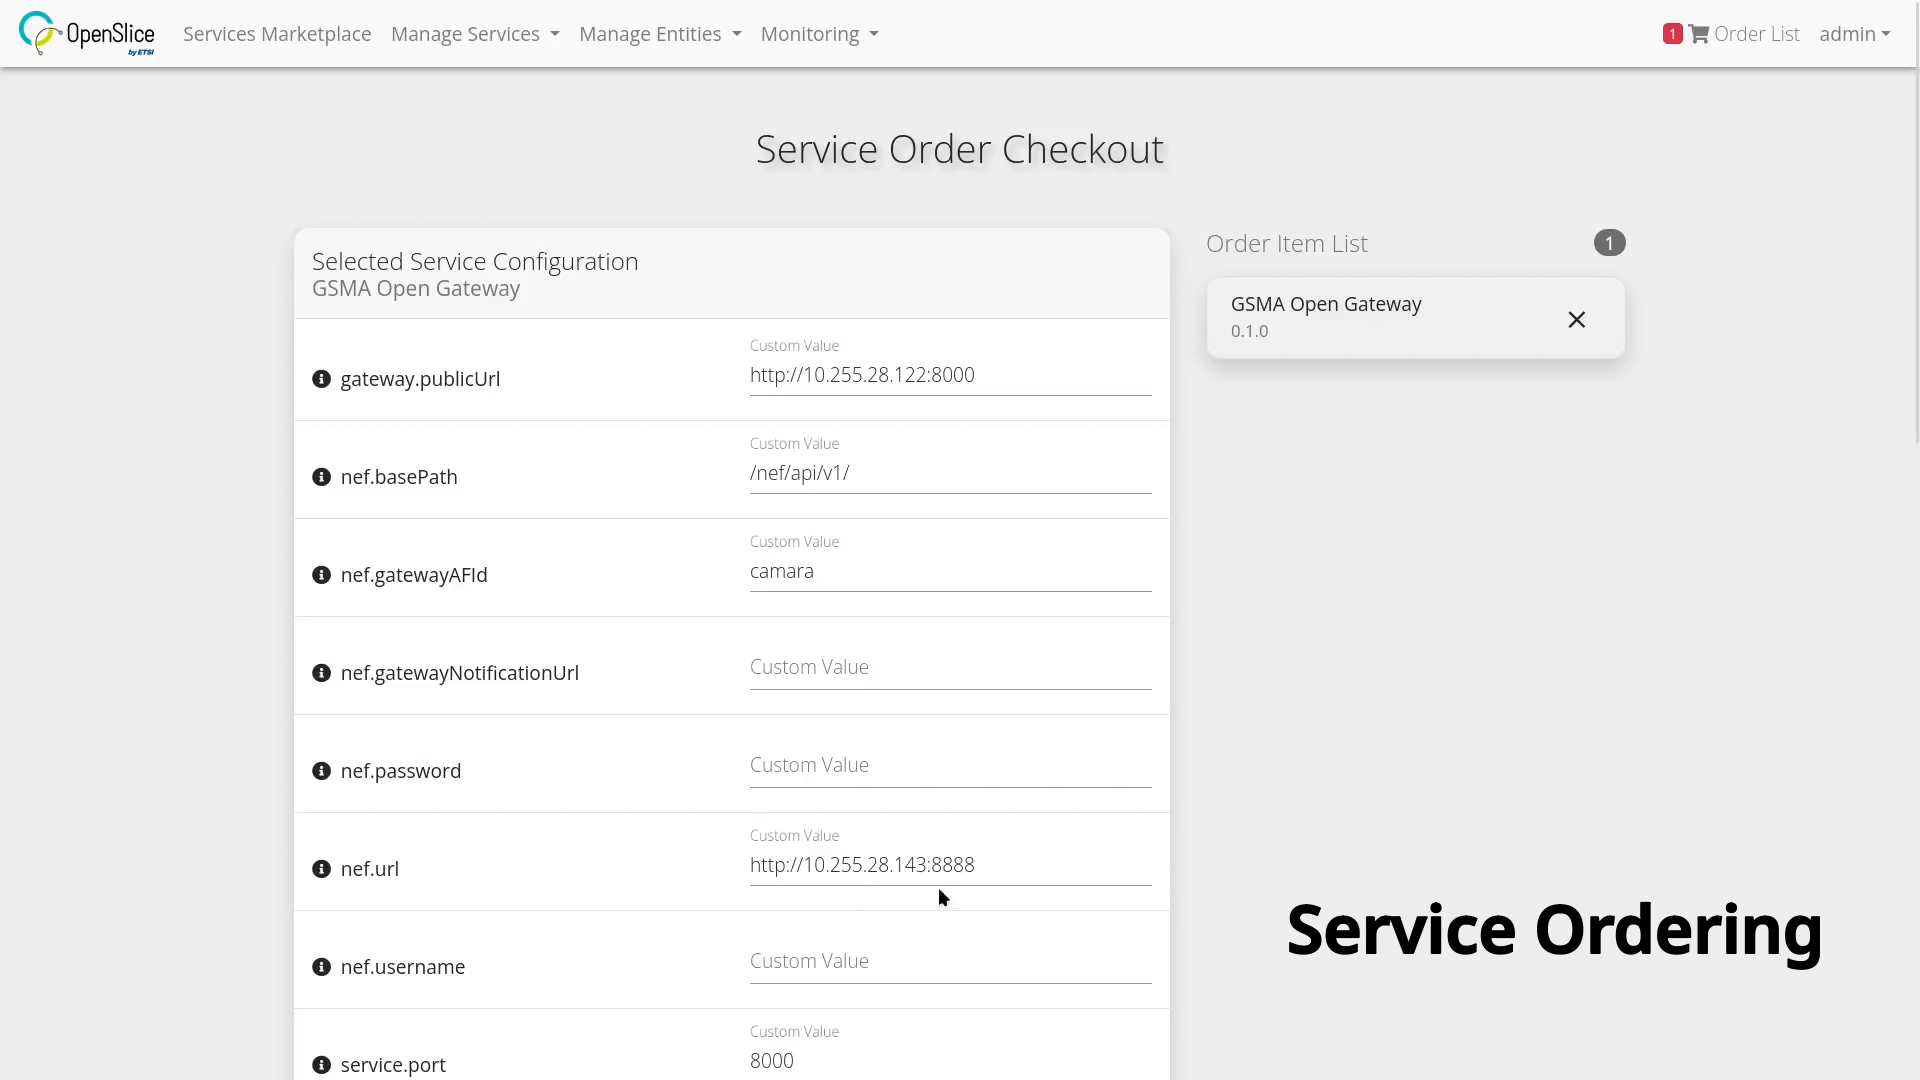
\includegraphics[width=\textwidth]{figs/osl_service_order.png}
	\caption{Screenshot of the user ordering the service}
\end{figure}
